% ═══════════════════════════════════════════════════════════════════════
%  Meridian — Milestone 2 Standalone Report
%  CSE 345/545 Foundations of Computer Security
%  Compile: pdflatex milestone2_report.tex (run twice for TOC)
% ═══════════════════════════════════════════════════════════════════════
\documentclass[12pt, a4paper]{article}

% ─── Packages ─────────────────────────────────────────────────────────
\usepackage[utf8]{inputenc}
\usepackage[T1]{fontenc}
\usepackage{lmodern}
\usepackage[margin=1in]{geometry}
\usepackage{graphicx}
\usepackage{hyperref}
\usepackage{xcolor}
\usepackage{listings}
\usepackage{booktabs}
\usepackage{enumitem}
\usepackage{fancyhdr}
\usepackage{titlesec}
\usepackage{float}
\usepackage{caption}
\usepackage{subcaption}
\usepackage{amsmath}
\usepackage{amssymb}
\usepackage{tikz}

% ─── Colors ───────────────────────────────────────────────────────────
\definecolor{meridianblue}{HTML}{4F46E5}
\definecolor{meridiandark}{HTML}{1E1B4B}
\definecolor{codebg}{HTML}{F8F9FA}
\definecolor{codeframe}{HTML}{D1D5DB}

% ─── Hyperref ─────────────────────────────────────────────────────────
\hypersetup{
    colorlinks=true,
    linkcolor=meridianblue,
    urlcolor=meridianblue,
    pdfauthor={Team Meridian},
    pdftitle={Meridian — Milestone 2 Report},
    pdfsubject={CSE 345/545 Course Project — Milestone 2},
}

% ─── Code listings ───────────────────────────────────────────────────
\lstset{
    basicstyle=\ttfamily\small,
    backgroundcolor=\color{codebg},
    frame=single,
    rulecolor=\color{codeframe},
    breaklines=true,
    captionpos=b,
    tabsize=2,
    showstringspaces=false,
    keywordstyle=\color{meridianblue}\bfseries,
    commentstyle=\color{gray},
    stringstyle=\color{red!70!black},
}

% ─── Headers & footers ──────────────────────────────────────────────
\pagestyle{fancy}
\fancyhf{}
\fancyhead[L]{\small\textcolor{gray}{CSE 345/545 — Milestone 2}}
\fancyhead[R]{\small\textcolor{gray}{Meridian}}
\fancyfoot[C]{\thepage}
\renewcommand{\headrulewidth}{0.4pt}

% ─── Section styling ────────────────────────────────────────────────
\titleformat{\section}
    {\Large\bfseries\color{meridiandark}}
    {\thesection}{1em}{}
\titleformat{\subsection}
    {\large\bfseries\color{meridiandark}}
    {\thesubsection}{1em}{}
\titleformat{\subsubsection}
    {\normalsize\bfseries\color{meridiandark}}
    {\thesubsubsection}{1em}{}

\graphicspath{{../../report/figures/}}

% ═══════════════════════════════════════════════════════════════════════
\begin{document}

% ─── Title Page ──────────────────────────────────────────────────────
\begin{titlepage}
    \centering
    \vspace*{2cm}

    {\Huge\bfseries\textcolor{meridiandark}{Meridian}\par}
    \vspace{0.5cm}
    {\Large\textcolor{meridianblue}{Secure Job Search \& Professional\\Networking Platform}\par}

    \vspace{1.5cm}

    {\LARGE\textbf{Milestone 2 Report}\par}
    \vspace{0.3cm}
    {\large Authentication, 2FA, Profiles, Resume Encryption, Admin\par}

    \vspace{1.5cm}

    {\large\textbf{CSE 345/545 — Foundations of Computer Security}\par}

    \vspace{1.5cm}

    \begin{tabular}{ll}
        \toprule
        \textbf{Team Members} & \textbf{Roll Number} \\
        \midrule
        Aniket Gupta    & 2022073 \\
        Angadjeet Singh & 2022071 \\
        Harsh Kumar     & 2022198 \\
        \bottomrule
    \end{tabular}

    \vspace{2cm}

    {\large IIIT Delhi\par}
    {\large February 27, 2026\par}
\end{titlepage}

% ─── Table of Contents ──────────────────────────────────────────────
\newpage
\tableofcontents
\newpage

% ═══════════════════════════════════════════════════════════════════════
%  1. Overview — What this milestone covers
% ═══════════════════════════════════════════════════════════════════════
\section{Overview}

This report covers Milestone~2 of the Meridian platform, due February~27, 2026. The milestone required five deliverables:

\begin{enumerate}
    \item Secure user registration and login
    \item TOTP-based two-factor authentication (replacing email OTP per instructor guidance)
    \item User profile management
    \item Secure resume upload with encryption at rest
    \item Basic admin dashboard
\end{enumerate}

All five goals are fully implemented and tested. This report details each goal's design, implementation, and security rationale, followed by a summary of the security measures protecting the platform.

\subsection{Technology Stack}

\begin{table}[H]
\centering
\small
\begin{tabular}{p{3cm} p{4cm} p{6cm}}
    \toprule
    \textbf{Layer} & \textbf{Technology} & \textbf{Rationale} \\
    \midrule
    Backend & Python / FastAPI & Async, auto-docs, Pydantic validation, dependency injection \\
    Frontend & React 18 / Vite & Component reuse, JSX auto-escaping (XSS defense) \\
    Database & PostgreSQL 16 & UUID support, JSONB for audit details, ACID compliance \\
    Deployment & Docker + GitHub Actions & Reproducible builds, automated CI/CD \\
    \bottomrule
\end{tabular}
\end{table}

\subsection{Architecture}

\begin{center}
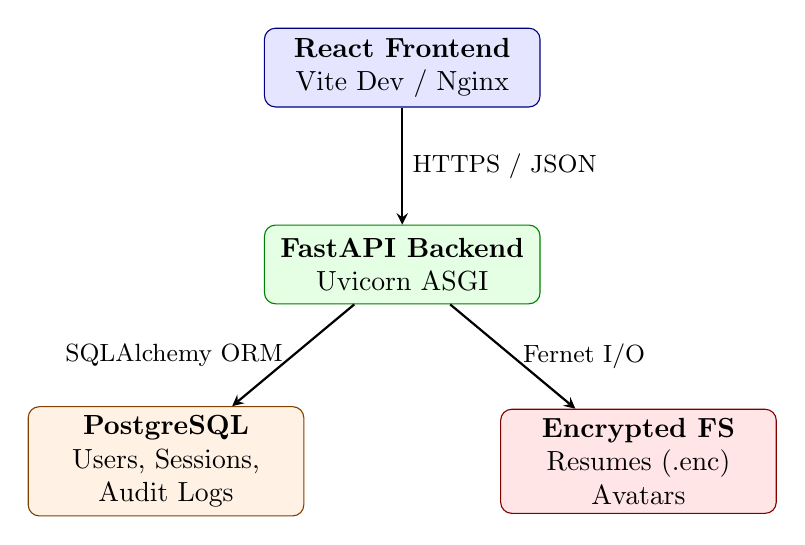
\begin{tikzpicture}[
    box/.style={draw, rounded corners, minimum width=3.5cm, minimum height=1cm, align=center, fill=#1!10, draw=#1!50!black},
    arrow/.style={->, thick, >=stealth}
]
    \node[box=blue] (client) at (0, 6) {\textbf{React Frontend}\\Vite Dev / Nginx};
    \node[box=green] (api) at (0, 3.5) {\textbf{FastAPI Backend}\\Uvicorn ASGI};
    \node[box=orange] (db) at (-3, 1) {\textbf{PostgreSQL}\\Users, Sessions,\\Audit Logs};
    \node[box=red] (fs) at (3, 1) {\textbf{Encrypted FS}\\Resumes (.enc)\\Avatars};
    \draw[arrow] (client) -- node[right, font=\small] {HTTPS / JSON} (api);
    \draw[arrow] (api) -- node[left, font=\small] {SQLAlchemy ORM} (db);
    \draw[arrow] (api) -- node[right, font=\small] {Fernet I/O} (fs);
\end{tikzpicture}
\end{center}

% ═══════════════════════════════════════════════════════════════════════
%  2–6. The five goals — reuse the shared milestone2.tex content
% ═══════════════════════════════════════════════════════════════════════
% ═══════════════════════════════════════════════════════════════════════
%  Section 5 — Milestone 2 (Main Deliverable)
% ═══════════════════════════════════════════════════════════════════════

\section{Milestone 2 — Authentication, Profiles, Resumes, Admin}
\label{sec:milestone2}

This milestone transforms the skeleton from M1 into a functional, security-hardened platform. It delivers five interconnected goals: secure authentication, TOTP-based 2FA, profile management, encrypted resume upload, and an admin dashboard. Each goal builds on the previous — authentication protects profiles, profiles hold resumes, and the admin dashboard oversees everything.

% ─────────────────────────────────────────────────────────────────────
\subsection{Goal 1: Secure Authentication}

Authentication is the front door to every other feature, so we invested heavily in making it resilient.

\subsubsection{Registration}

When a user registers, their password goes through \textbf{Argon2id} hashing — a memory-hard algorithm designed to resist GPU-based cracking. We configure it with 64~MB memory cost, 3 iterations, and 4 parallel threads. The system also validates password strength (minimum 8 characters, mixed case, digits, and symbols) and rejects common passwords before hashing.

To prevent email enumeration, failed registrations return a generic error regardless of whether the email already exists.

\subsubsection{Login}

The login flow incorporates several defenses that work together:

\begin{enumerate}
    \item \textbf{CSRF check} — The double-submit cookie pattern verifies the request is genuine.
    \item \textbf{Lockout check} — After 5 failed attempts, the account locks for 15 minutes.
    \item \textbf{Timing-safe verification} — If the email doesn't exist, we still compute a dummy Argon2 hash to prevent timing-based enumeration.
    \item \textbf{2FA branch} — If TOTP is enabled, a short-lived temp token (5 min) is returned instead of session cookies. The user must verify with their authenticator app before gaining access.
\end{enumerate}

On successful login, a database session is created with a device fingerprint (hashed IP + User-Agent) bound to the token. This means a stolen JWT cannot be used from a different device.

\subsubsection{Token Architecture}

We use a dual-token system stored exclusively in HttpOnly cookies — never in localStorage:

\begin{itemize}
    \item \textbf{Access token} (15 min TTL) — Carries user ID, role, session ID, and device fingerprint. Used for API authorization.
    \item \textbf{Refresh token} (24h TTL) — Scoped to \texttt{/api/auth/refresh}. Contains a unique JTI that rotates on every refresh.
\end{itemize}

If a previously-used JTI appears (suggesting token theft), \textbf{all of that user's sessions are immediately revoked} — a defense inspired by OAuth~2.0 refresh token rotation best practices.

% ─────────────────────────────────────────────────────────────────────
\subsection{Goal 2: TOTP Two-Factor Authentication}

Per instructor guidance, we implement TOTP (RFC~6238) rather than email/SMS OTP. This has practical advantages: it works offline, is compatible with standard authenticator apps (Google Authenticator, Authy), and requires no third-party SMS provider.

\subsubsection{Setup}

The setup process is designed to prevent accidental lock-outs:

\begin{enumerate}
    \item The backend generates a random Base32 secret using \texttt{pyotp}.
    \item The secret is \textbf{Fernet-encrypted} before being stored in the database — even a database breach won't expose TOTP seeds.
    \item A QR code is generated from the \texttt{otpauth://} URI and sent to the frontend as Base64-encoded PNG.
    \item The user scans the QR code and must \textit{confirm} by entering a valid code.
    \item Only after confirmation is 2FA activated. This prevents the user from enabling 2FA without actually setting up their authenticator.
\end{enumerate}

\subsubsection{Replay Prevention}

A valid TOTP code is reusable within its 30-second window, which opens a replay attack vector. We close it by recording every verified code in a \texttt{used\_otps} table with its time step. Before accepting a code, the system checks if it's been used in the current or adjacent windows (to account for clock drift). Old entries are garbage-collected after 5 minutes.

% ─────────────────────────────────────────────────────────────────────
\subsection{Goal 3: User Profile Management}

With authentication in place, users can build their professional profiles.

\subsubsection{Profile Data}

The profile supports rich professional information: name, headline, location, bio, education history, work experience, and skills. Education and experience entries support full CRUD operations, while skills use an autocomplete interface backed by a curated list of 150+ professional skills.

\subsubsection{Input Sanitization}

Every text field passes through a sanitizer that strips HTML tags (via \texttt{bleach}), removes JavaScript event handlers, and blocks \texttt{javascript:} URIs. This server-side sanitization, combined with React's automatic JSX escaping on the client, creates a two-layer XSS defense.

\subsubsection{Avatar Security}

Profile pictures go through a validation pipeline that goes beyond simple extension checking:

\begin{enumerate}
    \item Extension whitelist (\texttt{.jpg}, \texttt{.jpeg}, \texttt{.png})
    \item MIME type verification
    \item \textbf{Magic byte validation} — the first bytes must match JPEG (\texttt{FF D8 FF}) or PNG (\texttt{89 50 4E 47}) signatures, preventing disguised file attacks
    \item 2~MB size cap
    \item UUID-based filename — the original name never reaches the filesystem
\end{enumerate}

% ─────────────────────────────────────────────────────────────────────
\subsection{Goal 4: Encrypted Resume Storage}

Resumes are the most sensitive data on the platform. A breach that exposes plaintext resumes would compromise names, addresses, phone numbers, and career histories of every user. Our approach ensures that even if an attacker gains filesystem access, the data remains encrypted.

\subsubsection{The Upload Pipeline}

Uploads go through a multi-stage process before reaching disk:

\begin{enumerate}
    \item \textbf{Validation} — Extension (\texttt{.pdf}), MIME type (\texttt{application/pdf}), magic bytes (\texttt{\%PDF-}), size (2~MB limit), and content scan for suspicious embedded JavaScript, \texttt{/Launch}, and \texttt{/OpenAction} commands.
    \item \textbf{Encryption} — The validated content is encrypted with \textbf{Fernet} (AES-128-CBC + HMAC-SHA256). The encryption key is a 256-bit key stored in an environment variable, never in code.
    \item \textbf{Storage} — Written as \texttt{<uuid>.enc} on disk. The original filename exists only in the database.
\end{enumerate}

\subsubsection{The Download Pipeline}

On download, the process reverses — but critically, the decrypted content \textbf{never touches disk}. It's decrypted in memory and streamed directly to the client over HTTPS. Every download is recorded in the audit log.

\subsubsection{Verification}

Encrypted files on disk are completely unreadable without the key. Examining a stored resume shows only the Fernet token (starting with \texttt{gAAA...}), confirming that no plaintext leaks to the filesystem.

% ─────────────────────────────────────────────────────────────────────
\subsection{Goal 5: Admin Dashboard}

The admin dashboard provides platform-wide visibility and control. Admins can list all users, change roles, suspend accounts (which immediately revokes all active sessions), and permanently delete users (cascading to resumes, sessions, and OTP records).

All admin actions — especially destructive ones like deletion — are logged in the audit trail with the admin's identity and the target user's details. This creates accountability even for privileged users.

\subsubsection{Audit Events}

The system logs over 20 distinct event types, including: registration, login success/failure, 2FA setup, account lockout, resume upload/download/deletion, role changes, suspensions, and — importantly — \texttt{refresh\_token\_reuse\_detected}, which signals a potential token theft incident.

Each event captures the timestamp, actor ID, client IP, and a JSONB payload with contextual details specific to that event type.

% ─────────────────────────────────────────────────────────────────────
\subsection{User Interface}

The frontend uses a dark theme with glassmorphism design and smooth animations. Below are screenshots of the key interfaces delivered in Milestone~2.

\begin{figure}[H]
    \centering
    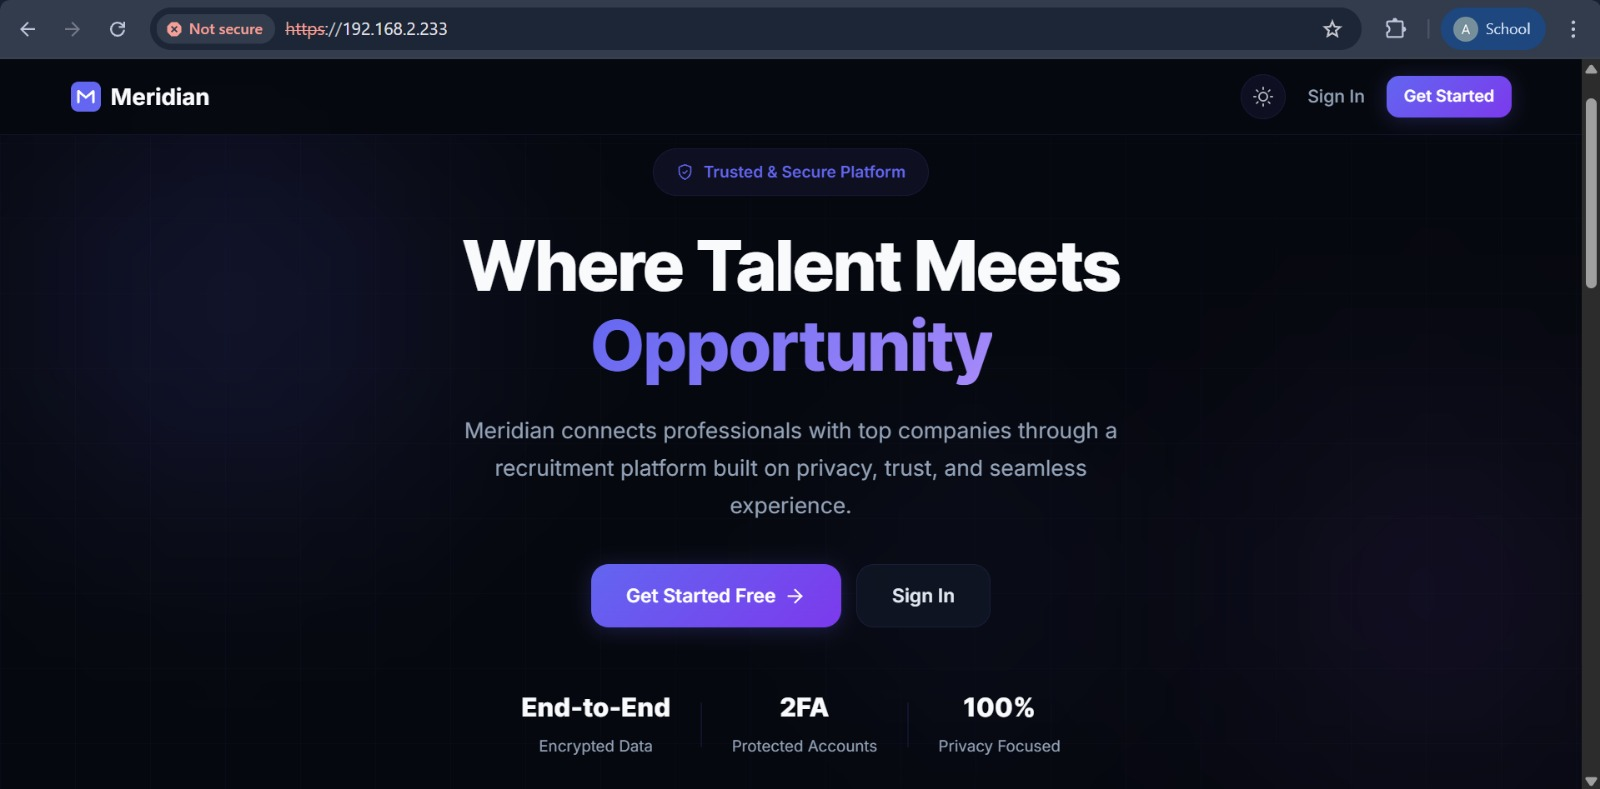
\includegraphics[width=\textwidth]{landing_page_1.png}
    \caption{Landing page — hero section with value proposition and security highlights.}
    \label{fig:landing1}
\end{figure}

\begin{figure}[H]
    \centering
    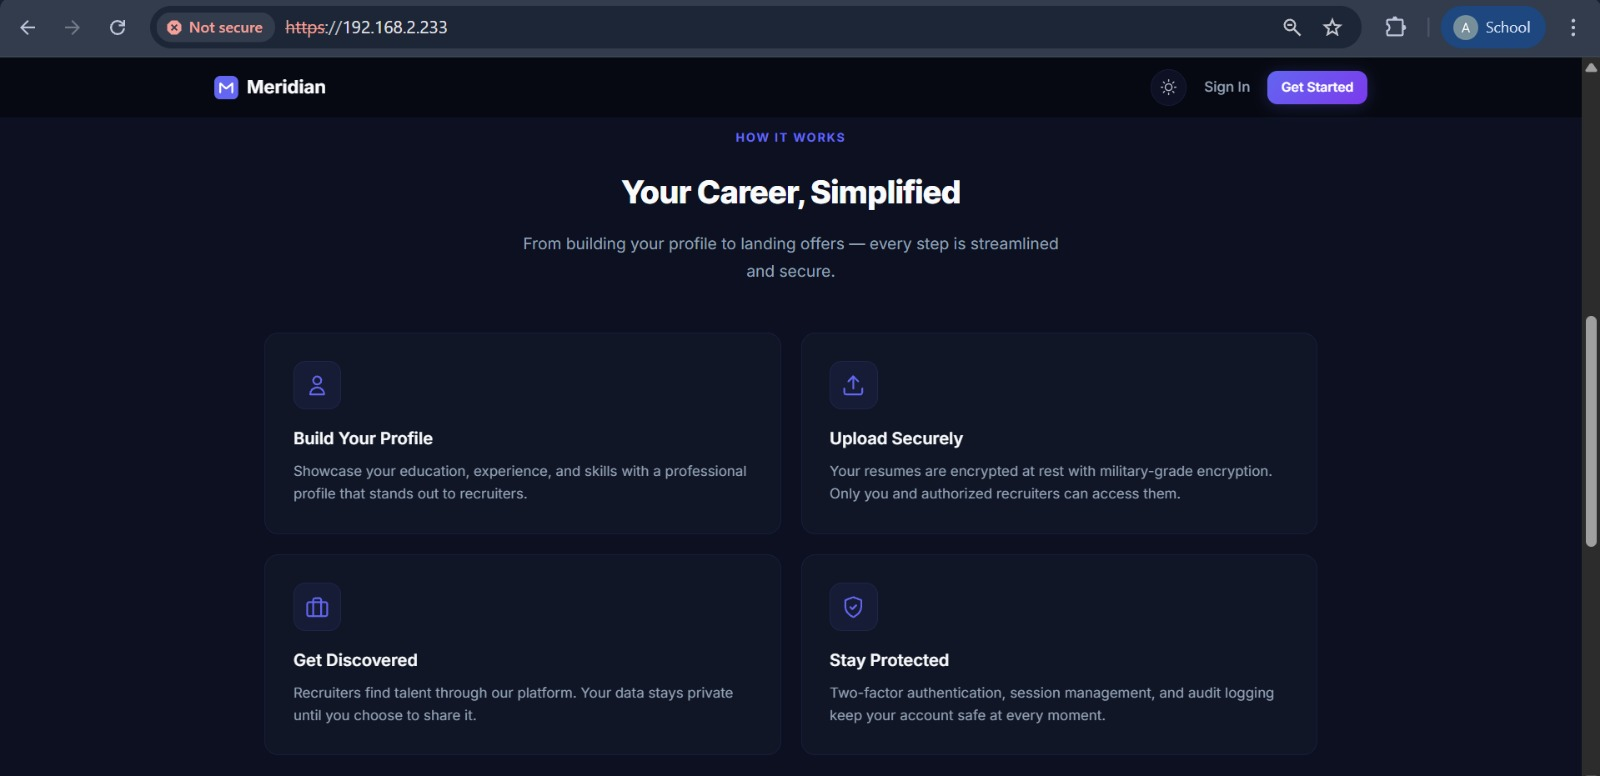
\includegraphics[width=\textwidth]{landing_page_2.png}
    \caption{Landing page — feature cards highlighting encryption, 2FA, and audit capabilities.}
    \label{fig:landing2}
\end{figure}

\begin{figure}[H]
    \centering
    \begin{subfigure}{0.48\textwidth}
        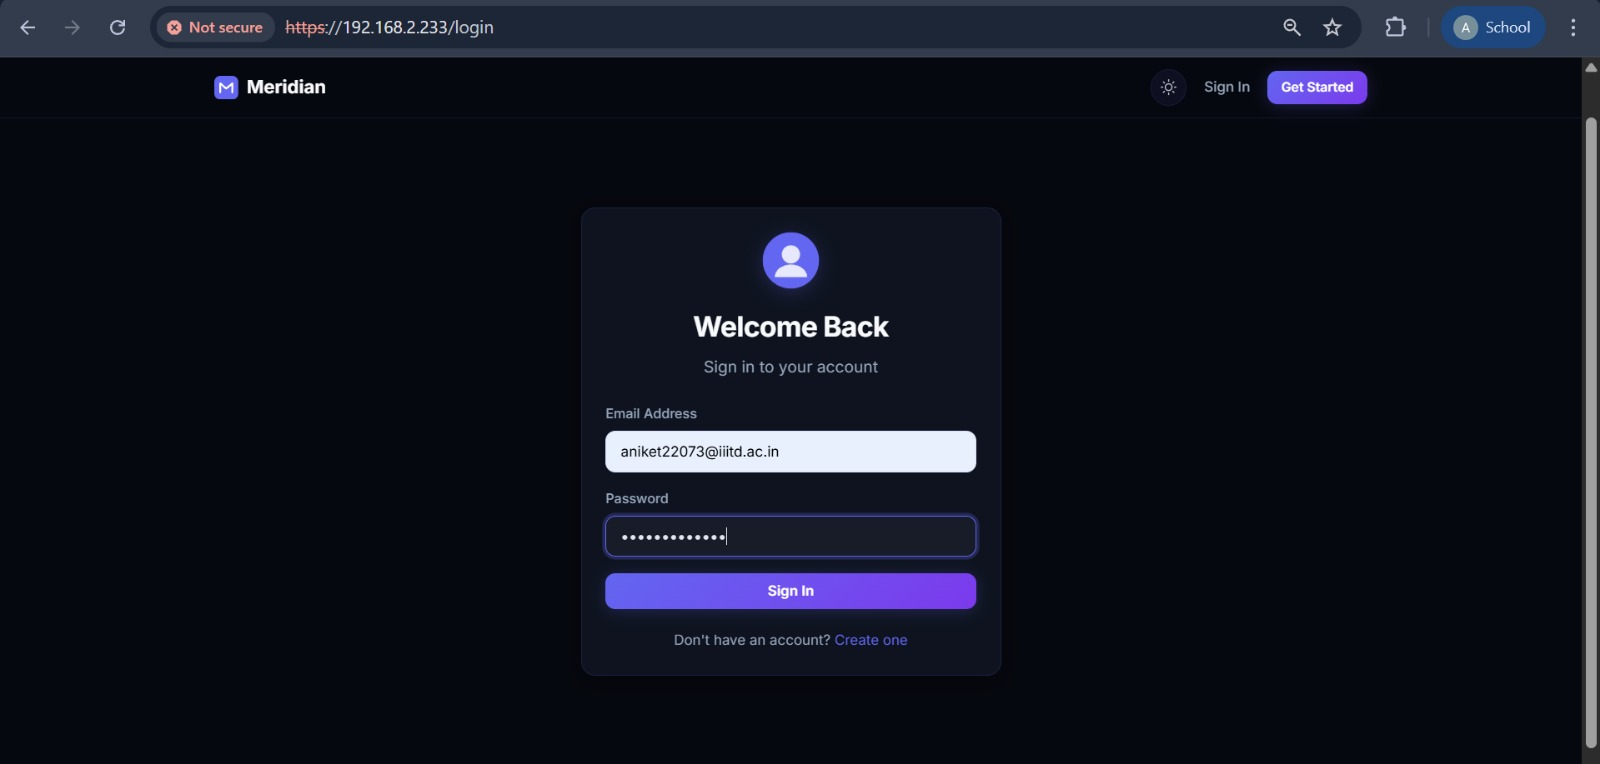
\includegraphics[width=\textwidth]{register.png}
        \caption{Login page}
        \label{fig:login}
    \end{subfigure}
    \hfill
    \begin{subfigure}{0.48\textwidth}
        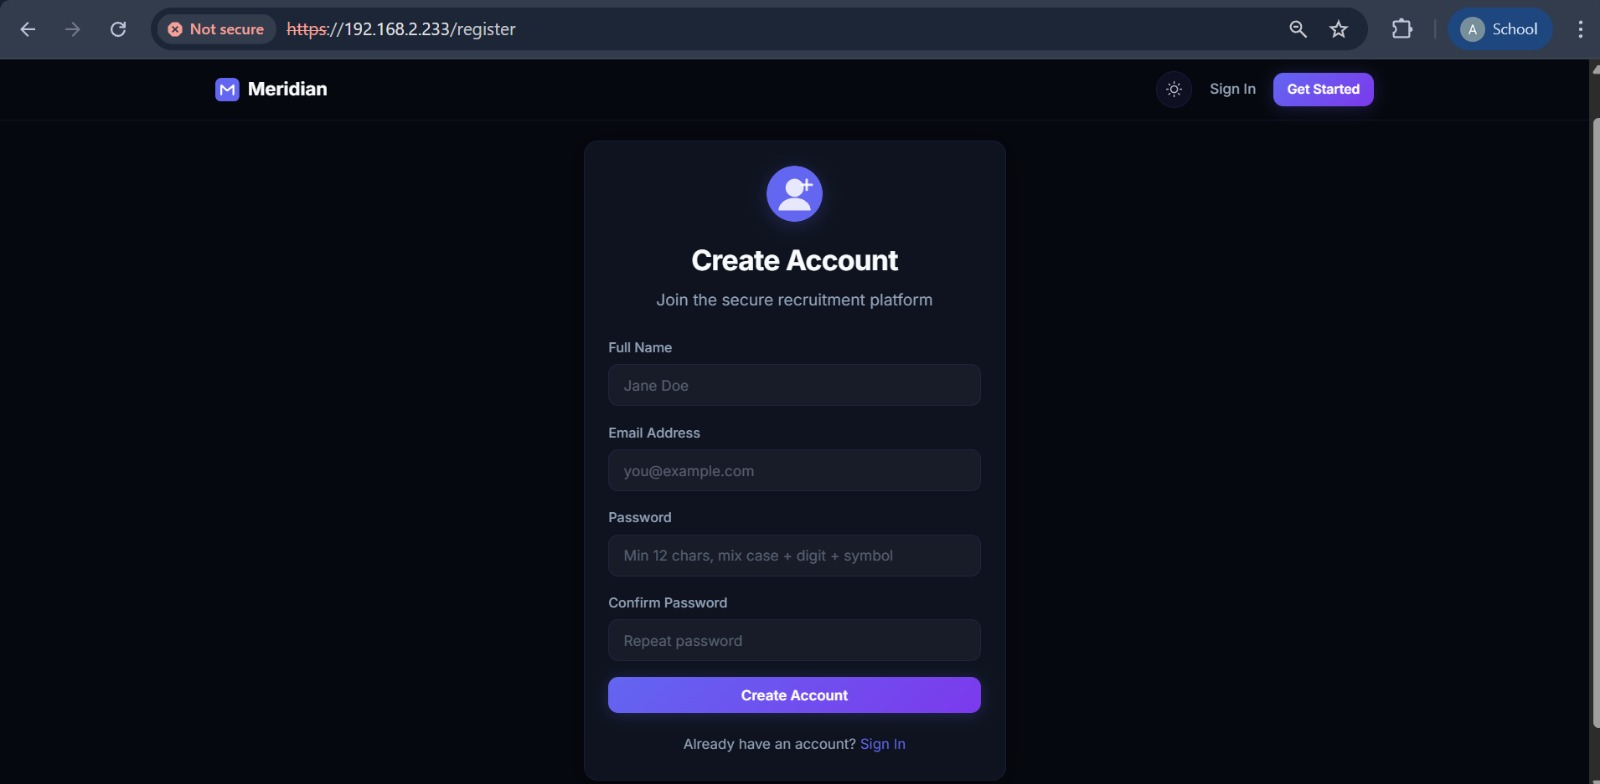
\includegraphics[width=\textwidth]{signup.png}
        \caption{Registration page}
        \label{fig:register}
    \end{subfigure}
    \caption{Authentication pages with gradient avatars and glassmorphism cards.}
\end{figure}

\begin{figure}[H]
    \centering
    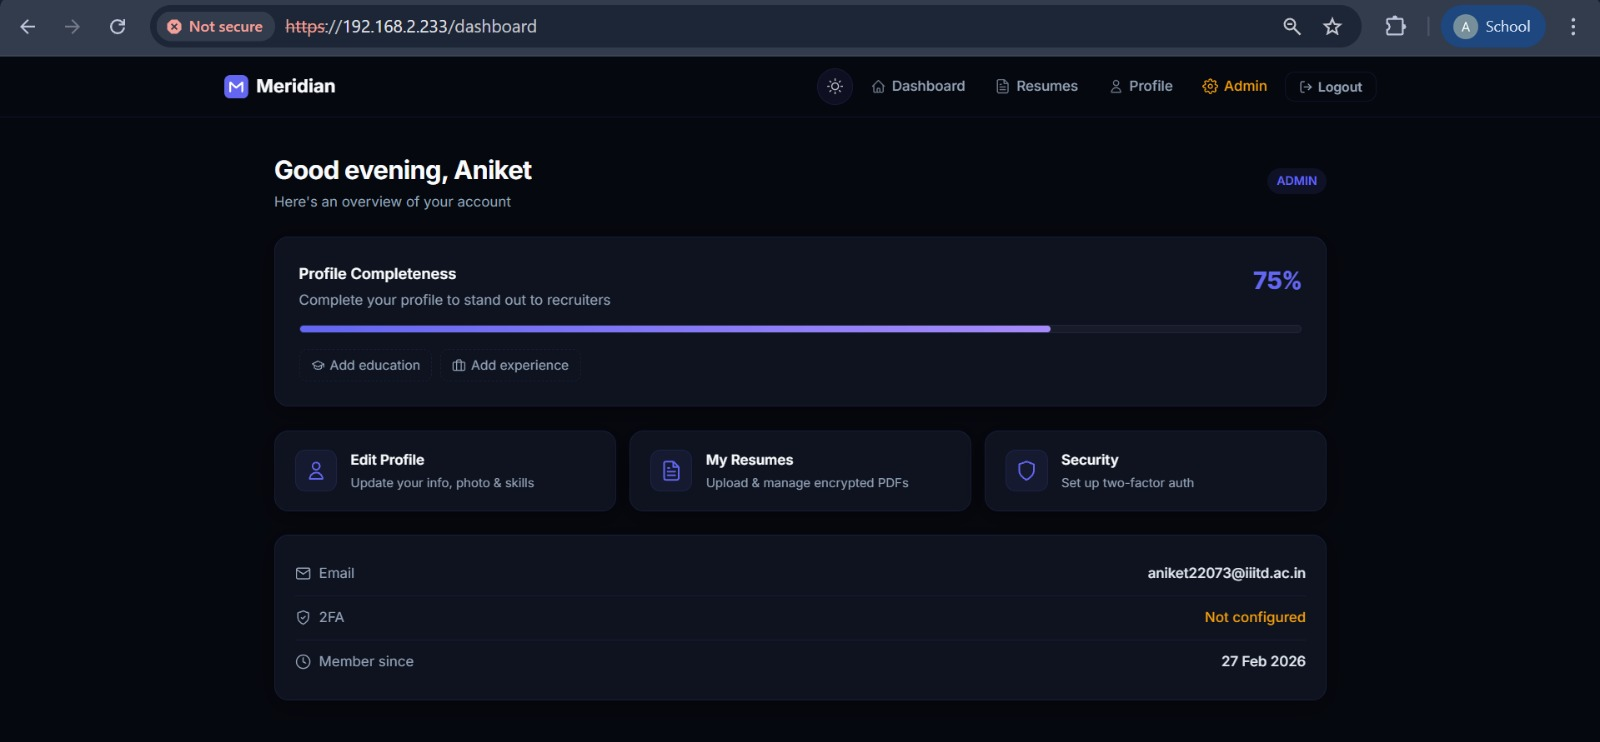
\includegraphics[width=\textwidth]{dashboard.png}
    \caption{Dashboard — profile completeness indicator, quick actions, and account summary.}
    \label{fig:dashboard}
\end{figure}

\begin{figure}[H]
    \centering
    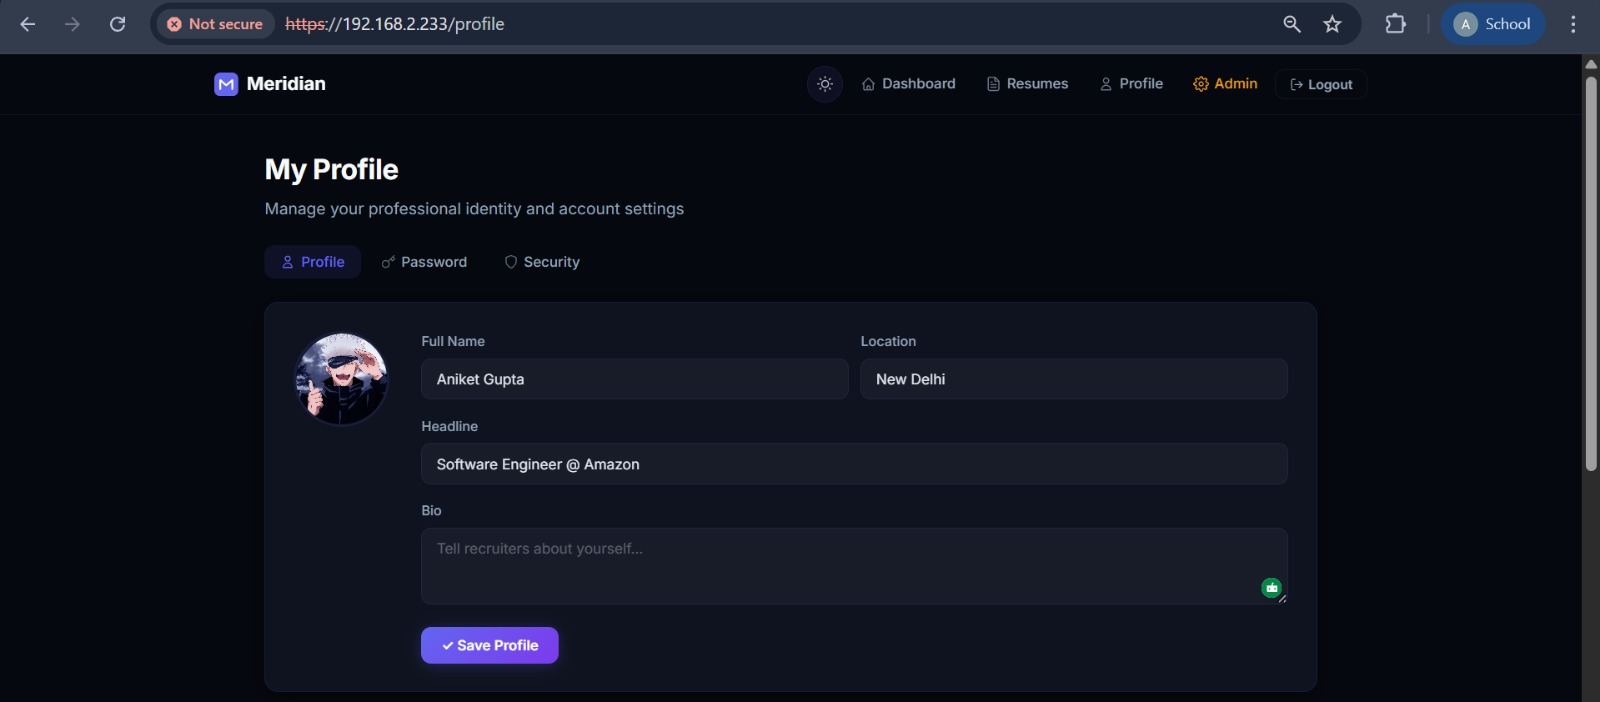
\includegraphics[width=\textwidth]{profile.png}
    \caption{Profile management — education, experience, and skills with inline editing.}
    \label{fig:profile}
\end{figure}

\begin{figure}[H]
    \centering
    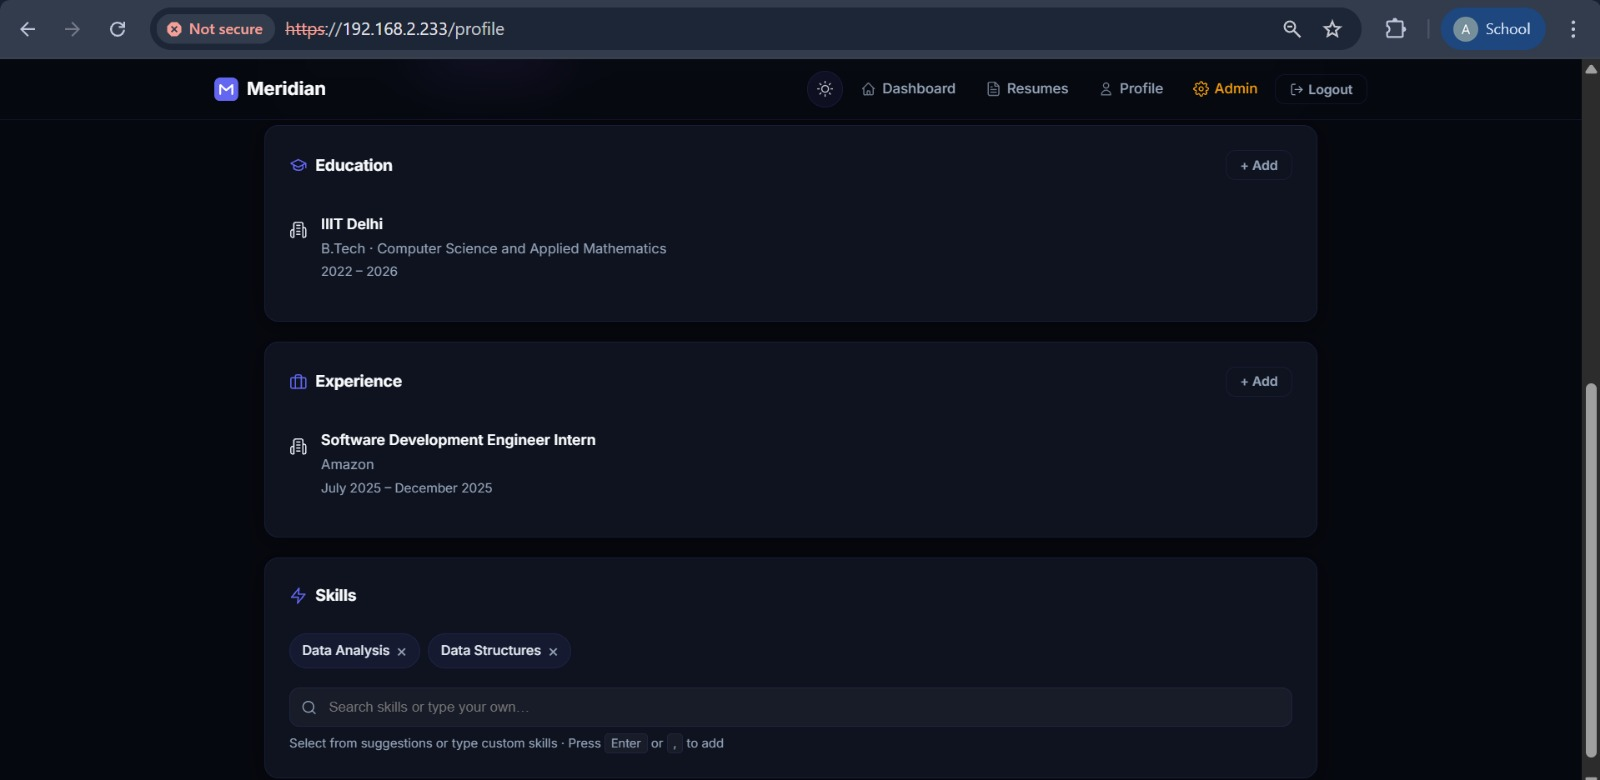
\includegraphics[width=\textwidth]{user_fields.png}
    \caption{Profile fields — sanitized text inputs with real-time validation.}
    \label{fig:userfields}
\end{figure}

\begin{figure}[H]
    \centering
    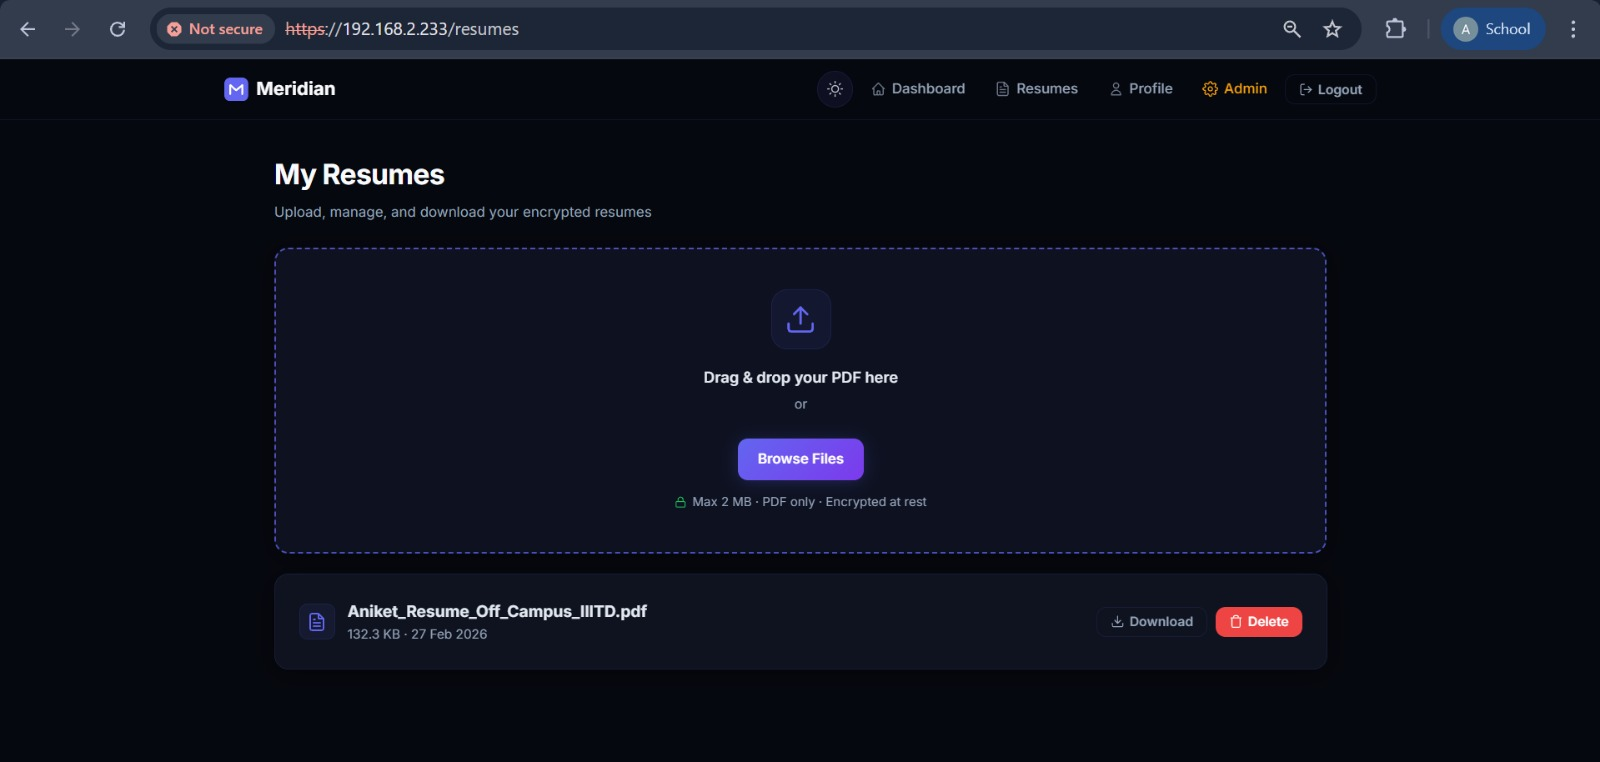
\includegraphics[width=\textwidth]{resume.png}
    \caption{Resume management — encrypted upload, listing, and secure download.}
    \label{fig:resume}
\end{figure}

\begin{figure}[H]
    \centering
    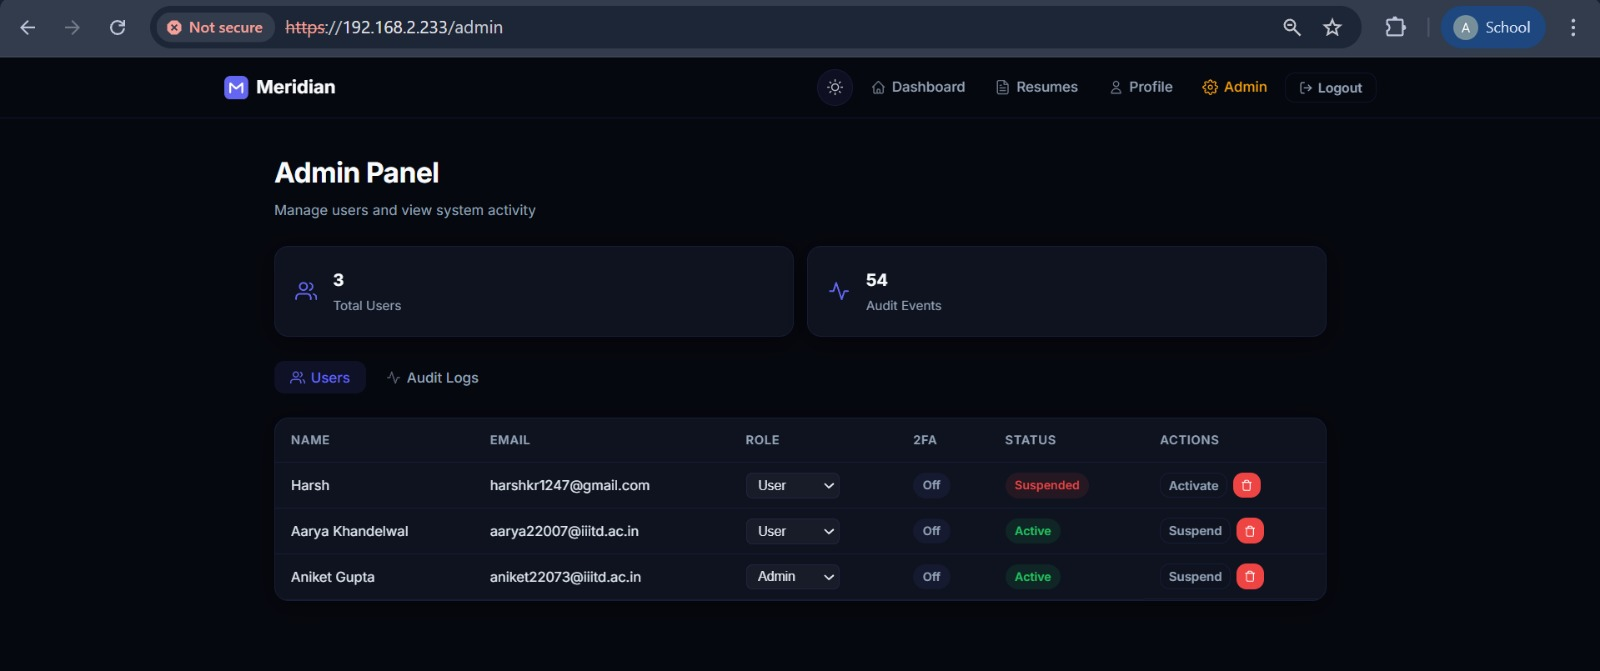
\includegraphics[width=\textwidth]{admin_panel.png}
    \caption{Admin panel — user management with role promotion, suspension, and deletion.}
    \label{fig:admin}
\end{figure}

\begin{figure}[H]
    \centering
    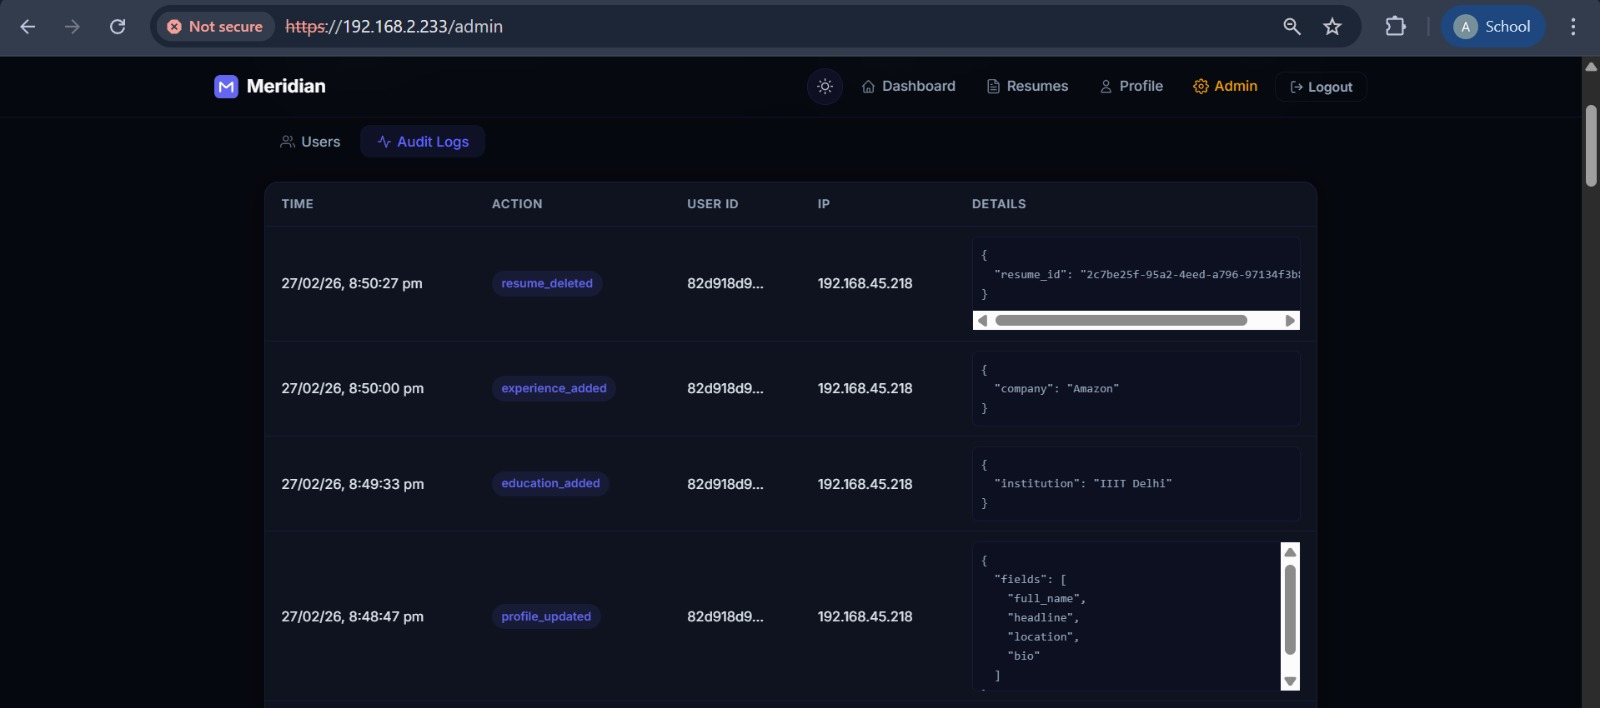
\includegraphics[width=\textwidth]{audits.png}
    \caption{Audit logs — every security event with timestamp, actor, IP, and contextual details.}
    \label{fig:audits}
\end{figure}


% ═══════════════════════════════════════════════════════════════════════
%  Security Summary
% ═══════════════════════════════════════════════════════════════════════
\newpage
% ═══════════════════════════════════════════════════════════════════════
%  Section 6 — Security Measures
% ═══════════════════════════════════════════════════════════════════════

\section{Security Analysis}
\label{sec:security}

This section takes a threat-driven look at the platform's security posture. Rather than listing features in isolation, we examine each attack vector and explain how the architecture defends against it.

\subsection{Authentication Attacks}

\textbf{Password cracking.} Even if the database is compromised, passwords are protected by Argon2id with 64~MB memory cost — making GPU-based brute force prohibitively expensive. Each hash uses a unique 16-byte salt.

\textbf{Credential stuffing.} Automated login attempts from breached credentials are throttled by account lockout (5 attempts triggers a 15-minute lock). The lockout event is logged, alerting admins to potential attacks.

\textbf{User enumeration.} Both registration and login return generic error messages. On login with an unknown email, a dummy hash is computed to make the response time indistinguishable from a valid attempt.

\textbf{Token theft via XSS.} JWTs live in HttpOnly cookies — JavaScript cannot access them, even in a successful XSS scenario. Combined with server-side input sanitization and React's automatic escaping, XSS attack surface is minimal.

\textbf{Session hijacking.} Each token is bound to a device fingerprint (hash of IP + User-Agent). A stolen token used from a different device will be rejected. Additionally, refresh token rotation means a stolen refresh token can only be used once before the entire session graph is invalidated.

\subsection{Web Application Attacks}

\textbf{Cross-Site Scripting (XSS)} is mitigated at two layers. Server-side, \texttt{bleach.clean()} strips all HTML tags, event handlers, and JavaScript URIs from user input before storage. Client-side, React's JSX escaping prevents DOM injection. Security headers (\texttt{X-Content-Type-Options: nosniff}) prevent MIME-sniffing attacks.

\textbf{Cross-Site Request Forgery (CSRF)} is prevented via the double-submit cookie pattern. A random token is set as both a cookie and returned in the response body. State-changing requests must include the token in an \texttt{X-CSRF-Token} header, which must match the cookie. Since an attacker's site cannot read our cookies (same-origin policy), they cannot forge the header.

\textbf{SQL Injection} is structurally prevented — all queries use SQLAlchemy's ORM with parameterized bindings. No raw SQL strings exist in the codebase. Input validation via Pydantic schemas adds a second layer of defense.

\textbf{Session Fixation} is impossible because sessions are created server-side with fresh UUIDs. The client cannot influence session identifiers. On every login, a new session is created; on logout, the existing session is database-revoked.

\subsection{Data Protection}

Sensitive data is protected both in transit and at rest:

\begin{itemize}
    \item \textbf{Passwords} — Argon2id one-way hash (irreversible)
    \item \textbf{Resumes} — Fernet encryption on disk (AES-128-CBC + HMAC-SHA256); decrypted only in memory during authorized downloads
    \item \textbf{TOTP secrets} — Fernet-encrypted in the database; decrypted only during verification
    \item \textbf{Transport} — All traffic over HTTPS with TLS
\end{itemize}

File uploads face a five-layer validation pipeline (extension, MIME, magic bytes, size, content scan for PDFs) before encryption. Files are stored with UUID names to prevent path traversal, and the storage directory sits outside the web root.

\subsection{Access Control}

The RBAC model is enforced at the API layer, not the UI layer — meaning even if someone bypasses the frontend, the backend rejects unauthorized requests:

\begin{table}[H]
\centering
\small
\begin{tabular}{p{3cm} p{2.5cm} p{2.5cm} p{2.5cm}}
    \toprule
    \textbf{Resource} & \textbf{User} & \textbf{Recruiter} & \textbf{Admin} \\
    \midrule
    Own profile      & Read/Write & Read/Write & Read/Write \\
    Own resumes      & CRUD       & CRUD       & CRUD \\
    Others' resumes  & —          & Read       & Read \\
    User management  & —          & —          & Full \\
    Audit logs       & —          & —          & Read \\
    \bottomrule
\end{tabular}
\caption{RBAC permission matrix. Enforced via FastAPI \texttt{Depends()} injection.}
\end{table}

\subsection{Security Headers}

Every response includes hardened headers that defend against common browser-based attacks:

\begin{lstlisting}
X-Content-Type-Options: nosniff
X-Frame-Options: DENY
X-XSS-Protection: 1; mode=block
Strict-Transport-Security: max-age=31536000; includeSubDomains
Referrer-Policy: strict-origin-when-cross-origin
Content-Security-Policy: default-src 'self'; script-src 'self'; ...
Permissions-Policy: camera=(), microphone=(), geolocation=()
\end{lstlisting}


% ═══════════════════════════════════════════════════════════════════════
%  What's Next
% ═══════════════════════════════════════════════════════════════════════
\newpage
\section{What's Next — Milestone 3}

With the authentication and data protection foundation in place, Milestone~3 (March~31) will add:

\begin{itemize}
    \item Company pages and job postings (recruiter workflow)
    \item Job search with filters (keywords, location, remote, skills)
    \item Application tracking (Applied $\rightarrow$ Reviewed $\rightarrow$ Interviewed $\rightarrow$ Offer/Rejected)
    \item End-to-end encrypted 1:1 messaging between recruiters and candidates
    \item Expanded audit logging for all new features
\end{itemize}

\end{document}
